% $Id: template.tex 11 2007-04-03 22:25:53Z jpeltier $

\documentclass{vgtc}                          % final (conference style)
%\documentclass[review]{vgtc}                 % review
%\documentclass[widereview]{vgtc}             % wide-spaced review
%\documentclass[preprint]{vgtc}               % preprint
%\documentclass[electronic]{vgtc}             % electronic version

%% Uncomment one of the lines above depending on where your paper is
%% in the conference process. ``review'' and ``widereview'' are for review
%% submission, ``preprint'' is for pre-publication, and the final version
%% doesn't use a specific qualifier. Further, ``electronic'' includes
%% hyperreferences for more convenient online viewing.

%% Please use one of the ``review'' options in combination with the
%% assigned online id (see below) ONLY if your paper uses a double blind
%% review process. Some conferences, like IEEE Vis and InfoVis, have NOT
%% in the past.

%% Figures should be in CMYK or Grey scale format, otherwise, colour 
%% shifting may occur during the printing process.

%% These few lines make a distinction between latex and pdflatex calls and they
%% bring in essential packages for graphics and font handling.
%% Note that due to the \DeclareGraphicsExtensions{} call it is no longer necessary
%% to provide the the path and extension of a graphics file:
%% \includegraphics{diamondrule} is completely sufficient.
%%
\ifpdf%                                % if we use pdflatex
  \pdfoutput=1\relax                   % create PDFs from pdfLaTeX
  \pdfcompresslevel=9                  % PDF Compression
  \pdfoptionpdfminorversion=7          % create PDF 1.7
  \ExecuteOptions{pdftex}
  \usepackage{graphicx}                % allow us to embed graphics files
  \DeclareGraphicsExtensions{.pdf,.png,.jpg,.jpeg} % for pdflatex we expect .pdf, .png, or .jpg files
\else%                                 % else we use pure latex
  \ExecuteOptions{dvips}
  \usepackage{graphicx}                % allow us to embed graphics files
  \DeclareGraphicsExtensions{.eps}     % for pure latex we expect eps files
\fi%

%% it is recomended to use ``\autoref{sec:bla}'' instead of ``Fig.~\ref{sec:bla}''
\graphicspath{{figures/}{pictures/}{images/}{./}} % where to search for the images

\usepackage{microtype}                 % use micro-typography (slightly more compact, better to read)
\PassOptionsToPackage{warn}{textcomp}  % to address font issues with \textrightarrow
\usepackage{textcomp}                  % use better special symbols
\usepackage{mathptmx}                  % use matching math font
\usepackage{times}                     % we use Times as the main font
\renewcommand*\ttdefault{txtt}         % a nicer typewriter font
\usepackage{cite}                      % needed to automatically sort the references
\usepackage{tabu}                      % only used for the table example
\usepackage{booktabs}                  % only used for the table example
\usepackage{url}
\usepackage{float}
%% We encourage the use of mathptmx for consistent usage of times font
%% throughout the proceedings. However, if you encounter conflicts
%% with other math-related packages, you may want to disable it.


%% If you are submitting a paper to a conference for review with a double
%% blind reviewing process, please replace the value ``0'' below with your
%% OnlineID. Otherwise, you may safely leave it at ``0''.
\onlineid{0}

%% declare the category of your paper, only shown in review mode
\vgtccategory{Research}

%% allow for this line if you want the electronic option to work properly
\vgtcinsertpkg

%% In preprint mode you may define your own headline.
%\preprinttext{To appear in an IEEE VGTC sponsored conference.}

%% Paper title.

\title{An Efficient Language Learning Method-\\VR Vocabulary Crossword Puzzle Game}

%% This is how authors are specified in the conference style

%% Author and Affiliation (single author).
%%\author{Roy G. Biv\thanks{e-mail: roy.g.biv@aol.com}}
%%\affiliation{\scriptsize Allied Widgets Research}

%% Author and Affiliation (multiple authors with single affiliations).
\author{Jieqiong Li\thanks{e-mail: jacinda.li@colostate.edu} %
\and Zihui Li\thanks{e-mail:zihui.li@colostate.edu} %
\and Tianyi Xiong\thanks{e-mail:tianyi.xiong@colostate.edu}}
\affiliation{\scriptsize Colorado State University}

%% Author and Affiliation (multiple authors with multiple affiliations)
% \author{Jieqiong Li\thanks{e-mail: jacinda.li@colostate.edu}\\ %
%         \scriptsize Colorado State University %
% \and Zihui Li\thanks{e-mail:zihui.li@colostate.edu}\\ %
%      \scriptsize Colorado State University %
% \and Tianyi Xiong\thanks{e-mail:tianyi.xiong@colostate.edu}\\ %
%      \parbox{1.4in}{\scriptsize \centering Martha Colorado State University}}

%% A teaser figure can be included as follows, but is not recommended since
%% the space is now taken up by a full width abstract.
%\teaser{
%  \includegraphics[width=1.5in]{sample.eps}
%  \caption{Lookit! Lookit!}
%}

%% Abstract section.
\abstract{Human Computer Interaction (HCI) plays an significant role in modern education approaches. For most non-English native speaker, simply reciting English words written on books is inefficient because the nature learning curve of human brain makes people forget short-term memorized vocabulary very soon. Enlightened by English learners’ needs of long-term memorizing words and existing experimental results of scramble game, the authors novelly developed an VR vocabulary chess game based on human-machine interaction to boost gamer’s vocabulary efficiently as well as maintaining user stickiness. Experiment includes 2 groups that utilize VR cross word game, mixed learning method and real world recitation respectively. The result shows that VR cross game wins favor of most participants because it effectively stimulate learner's interest. We use ANOVA to analysis the result for getting the conclusion about which experiment is better from statistical perspective. It also performs better in long-term memorization than real-world recitation for English learners.
} % end of abstract

%% ACM Computing Classification System (CCS). 
%% See <http://www.acm.org/class/1998/> for details.
%% The ``\CCScat'' command takes four arguments.

\CCScatlist{ 
Virtual Reality, Language education, Game-based learning, Unity3D
}

%% Copyright space is enabled by default as required by guidelines.
%% It is disabled by the 'review' option or via the following command:
% \nocopyrightspace

%%%%%%%%%%%%%%%%%%%%%%%%%%%%%%%%%%%%%%%%%%%%%%%%%%%%%%%%%%%%%%%%
%%%%%%%%%%%%%%%%%%%%%% START OF THE PAPER %%%%%%%%%%%%%%%%%%%%%%
%%%%%%%%%%%%%%%%%%%%%%%%%%%%%%%%%%%%%%%%%%%%%%%%%%%%%%%%%%%%%%%%%

\begin{document}

%% The ``\maketitle'' command must be the first command after the
%% ``\begin{document}'' command. It prepares and prints the title block.

%% the only exception to this rule is the \firstsection command
%\firstsection{Introduction}

\maketitle

\section{Introduction} %for journal use above \firstsection{..} 

The utilization of Virtual Reality (VR) in education is relatively new method. VR offers the chance to make virtual objects bigger or smaller than it appears in reality. In addition, it help users jump out of the restrictions of time and real word physics, and make the invisible items visible, thus provide the sense of immersion to students/educators, help them interact with virtual objects or each other in new environment.

Immersion is a psychological state characterized by perceiving oneself to be enveloped by, included in, and interacting with an environment that provides a continuous stream of stimuli and experiences, making users feel immersed in an new virtual environment is a prerequisite for delightful experience.

Whether it is child education or adult education, there is no doubt that language learning is one of the most significant parts of education. Language education is an important education direction that can expand its horizons. As we all know, if a person wants to learn a new language, memorizing words is the first step in learning. However, some people still use the traditional methods to learn vocabulary, such as repeating words one by one, which also makes the learning language efficiency lower and lower. In addition, as a discipline that requires independent learning, if the student does not have enough interest to learn a new language, they will have high anxiety and pressure when reciting the vocabulary. How to make students more efficient and happier learning language will be the main goal of language education. 

The aim of this research is to combine the advantage of virtual reality technique and cross-word game in English education and develop a new method to help students learn English words more easily and happily. Moreover, it is necessary to verify the effectiveness of this new method and how effective it is in facilitating English learning. In this study ,we use the most influential technology - VR - to further enhance students' interest in learning. We have three purposes for this topic. First, we want to break traditional learning methods and improve the efficiency of students when reciting words. Second, we hope that when people use this game, they can be immersed in a more relaxed learning atmosphere, enjoy the fun of learning words. Last but not least, we hope that through the analysis of experimental results, we have learned whether VR technology has a good influence on education.

The key contributions of this article are as follows:
\begin{itemize}
\item We novelly develop a VR crossword puzzle game using well-designed alternative gaming and learning schema. We also proposed a lexicon allocation and vocabulary generation method to boost the efficiency of learning.
\item We are the first to compare the effectiveness of the VR crossword game in memorizing vocabulary with a real world learning method and half virtual half reality learning approach. The three group comparisons demonstrate the importance of VR in English education \cite{10.1145/257874.257886}. 
\end{itemize}

\begin{figure}[H]
 \centering 
 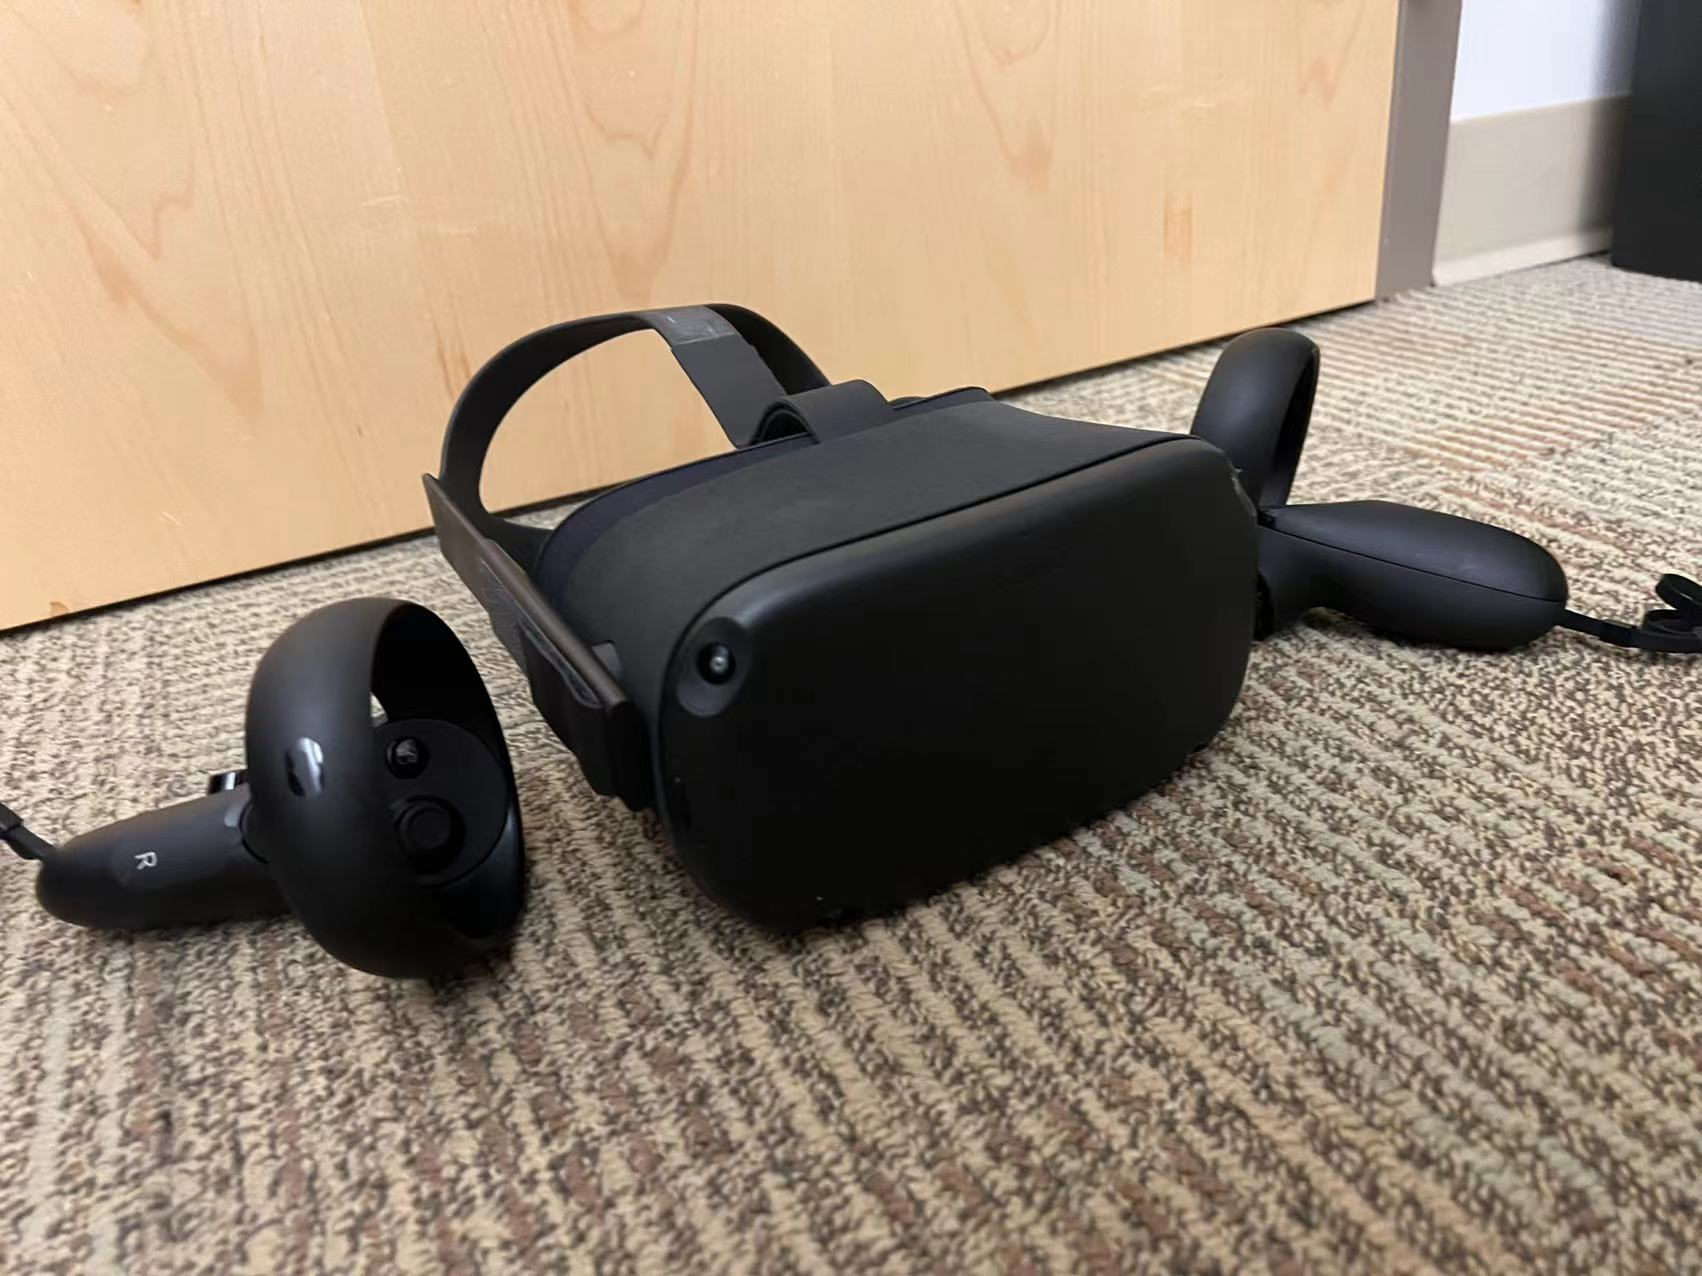
\includegraphics[width=\columnwidth]{pictures/OurOculus.jpg}
 \caption{The Oculus device used in this study.}
   \label{fig:oculus}
\end{figure}

\section{Motivation}
In 2019, Jing\cite{jing2019effectiveness} explains why students are anxious when learning languages. After we combined Jing’s discovery with our own learning experience, we found that learning methods and learning interests are the two main reasons that affect language learning. The first is the
problem of learning methods. Students need to have strong self-learning ability and perfect learning methods in order to learn a second language well. If students only learn the language by using the traditional method of memorizing words, they often fail to obtain a good result. 

Secondly, students will gradually lose interest in completing the boring task of reciting words. Therefore, we hope to create a game that can improve students' learning interests and learning efficiency to help students learn a second language happily. In the article, "The Effect of Puzzle Game on Students' Vocabulary Achievement Forum, Juliana (2020) explains the availability of crossword puzzle games for English teaching\cite{sitompul2020effect}. And Juliana points out that the game helps students raise their interests and helps to improve students' efficiency of the second language. She proposed that after using the crossword game, the students' vocabulary skill has obviously improved. 

In addition, the competition and time stress in the game will also give students more active in the process of playing games \cite{chang2003development}\cite{lin2007implementation}\cite{inkpen1995playing}. As the most popular 3D technology, VR technology is an optimal technology that attracts students and enhances students' interest in learning. 3D technology can help students improve their memory and implement an immersive learning environment \cite{billinghurst20122012}. As it was stated in \cite{yavoruk2019teaching}, XR provided a whole new state in 
helping students' learning ability. It has high potential in education field since XR utilize limited physical resources while can offer huge amount of virtual resources, the 3D rendering technique helps students learn the new knowledge in immersive environment. 

Since VR has advantages in fully utilize real world spaces and expand it in a immersed virtual world and has been proved to be an effective method in physics education. It is reasonable to infer that VR can serves as an effective teaching method in language study subjects such as English learning, targeting at
non-English native speaker.

The paper conducted an experiment which use VR technique to help students understand physical features of spheres. Result shows that students hold positive opinion toward VR implementation in real class. The goal of this study is to combine the crosswords and VR technologies, we will give students a new experience in reciting words and learning English. We also expect that by using this method, students will improve the ability to use a second language while playing games.

\section{Previous work}

Education has always been a hot topic. The researchers found that most students did not have high passion during their studies. To verify that the game can help students improve learning efficiency, in the article, "Puzzle Games on students' influence on non-English student vocabulary" Selly Novita Sitompul (2020) explains the effectiveness of the crossword in teaching \cite{sitompul2020effect}. This learning method can not only improve students 'learning efficiency but also reduce students' anxiety. The author also pointed out that this crossword can stimulate students' victory so that students are gradually familiar with the meaning of each word and spelling the process of spelling thoughts. 

In the article, "The face-to-face collaborative environment of the portable equipment in English Words”, Hong, Young, Lin (2009) explained the impact of the Crossword Game on learning efficiency under different platforms\cite{hung2009constructing}. They create experimental groups and control groups to prove that the use of computers to learn is better than using traditional ways.
As the most popular 3D technology, VR technology is the best technology to attract students and enhance students' interest in learning. Inman pointed out that in "VR Education and Rehabilitation" articles, VR technology brings good education development. Students may not focus on learning knowledge because they do not have a suitable learning environment and a good learning method\cite{inman1997vr}. 

In addition, high-intensity learning stress and low learning interest make students have anxious emotions during learning. Inman pointed out that VR technology allows students to be immersed in a more varied and interesting learning environment to help students learn more effectively\cite{alfadil2020effectiveness}. This is the main purpose of our choice of VR and games. We want to create a learning environment that can provide more relaxation and freedom. 

In the paper \cite{ying2017vrex}, the researchers proposed an education platform-VREX (Virtual Reality based Education eXpansion), which combined online and offline resources to improve learning experience for students from different level. The experiment results shows that VR was proved to be effective in promoting curriculum effectiveness by providing an immersive environment which facilitate students better understand abstract theory by forming virtual concrete 3D models and interacting with them while in real classroom these abstract theories are usually difficult for instructors to explain. This study also transformed slides from plane into VR scenes in order to let students feel immersed into an virtual relaxed environment. VREX adopt a multi-player interactive mode so every student would be able to communicate with teachers and classmates just as in physical classes anywhere at anytime or anywhere. VREX is designed to offer different level of education from K-12 to Universities, this study also provided actual statistical data as support material.

In 2017, the researchers \cite{marks2017getting} made an VR application aiming to help the medical students better understand and explore the nasal cavity structure and anatomy, this application presented a virtual 3D model of nasal cavity that can zoom in and zoom out, the design and evaluation processes were based on students' feedback. The experiment was positive and students have showed great interests toward VR anatomy, they also expect to improve the application with clearer images that distinguish inside and outside areas, they also expect smoother camera movement. Since VR already received positive feedback in natural science area, we infer that it may have similar effects to liberal art education.

In the paper \cite{singh2021virtual} Singh developed a VR‐based learning environment aiming for engineering students to manipulate the hardware equipment such as DSP filter in the electronics lab. The aim of this experimental study was to determine whether the use of VR technology in engineering laboratories is effective in improving students learning and cognition ability. The experimental results proved 
the hypothesis that VR technology has great positive effect on participant learning and cognition. 
This study also pointed out that immersion is an important factor when evaluate a VR system's performance. In this study, VLE provided a virtual DSP filter that looks same like real world equipment, and the behaviors that users made to the model is similar to the real equipment. The setup of this experiment offered the students an immersive environment, thus improved interactive learning experience. According to the feedback, students felt excited when doing the virtual laboratory equipment manipulation through VR technique. The students of the control group have showed more curiosity when learning through the VLE; most participants felt motivated to learn through the new VR technologies.

\section{Approach Overview and Methodology}
In this project, we will use Unity as a development platform and Virtual Reality techniques to build a vocabulary crossword game \cite{ebrahimi2017unity}. The project will be divided into 5 steps. 
First step is target population analysis. As described above, the population of non-English speakers is large, and the common learning obstacle is the amount of vocabulary a person can master. According to\cite{asgari2011type, gu2003vocabulary}, categorized vocabulary learning strategy helps learners memorize words faster by associating and grouping with other words. Thus we will adopt this strategy and apply the categorized learning method as baseline. Besides, traditional rote learning does not attract people any more, learning through VR applications has become \cite{alfadil2020effectiveness} a novel efficient approach which greatly increases user viscosity. 

Second phase is game designing. From the technical selection perspective, we use Oculus as a VR device, thus Unity becomes our first choice as a software platform since it provides Oculus SDKs \cite{bouvier2019advanced}. From the scientific point of view, we proposed a novel VR learning schema which proceeds learning and gaming alternatively with prompt feedback. We hypothesize this schema will boost the learning efficiency by using our well-designed word selection algorithm. The detailed game design process is as follows(R stands for the robot/system, U represent the user/gamer):
0. Before the start of the game, the system equally divides the words of the chosen category into 2 parts, then take one part (lexicon RL) as lexicon for the robot/machine/system, the other part(lexicon UL) as the alternative generative words prepared for users/gamers.

\begin{itemize}
    \item \textbf{Step1} - R starts first, choosing a word (wordRL)from the alternative lexicon and putting a virtual word on a pre-generated virtual chess board, each character occupying one chess grid.
    \item \textbf{Step2} - U choose characters from the set generated by the system(characterUL) from step 0, and put the word on the chessboard, making it cross with any of the words existing on the board.
    \item \textbf{Step3} - R selects a vocabulary from the lexicon RL, then puts that word on the chess board, intersecting with any of the vocabularies on board.

    \item \textbf{Step4} - Repeat steps 2 and 3 until time is up or the game is over. Here the end of the game means there is no available word that crosses with existing words while on the chess board.

    \item \textbf{Step5} - After each round of the game, there is a word learning section, U has to learn 5 words, each word will appear along with the 3D image of it’s physical object to help the user memorize faster and deeper.

    \item \textbf{Step6} - Proceed to the next round of the game.

    \item \textbf{Step7} - Repeat the above steps for several(2 or 3) times if applicable.
\end{itemize}

Third phase is the pre-test and post-test designing. 

\begin{table}[tb]
  \caption{Observation record}
  \label{tab:observation}
  \scriptsize%
	\centering%
  \begin{tabu}{%
	r%
	*{7}{c}%
	*{2}{r}%
	}
  \toprule
   ID & Words & Wrong number & Error Rate (ER) \\
  \midrule
   1 &  &  & & \\
   2 &  &  &  &\\
  \bottomrule
  \end{tabu}%
\end{table}


Before the experiment, game participants will be asked to take a topic-based vocabulary survey. E.g. If a user selects words about food and drinks as the topic, we’ll offer a word familiarity questionnaire about food, including the vocabulary they will learn in the game.

1- Design of the questionnaire. For each question, there will be three answers A,B,C indicating different levels of familiarity toward a word(see details \url{https://forms.office.com/r/HwakF9qHh9}): 
\begin{itemize}
\item A. Already mastered the word and can explain the meaning.
\item B. Seems familiar but doesn't know the exact meaning.
\item C. Don’t know the word.
\end{itemize}

2- Give weights to different answers. Option A = 2, option B = 1, score for option C is 0. Sum up the scores as the evaluation grade for that participant.

After the experiment, participants will be asked to take a similar survey. 
Compare the pre-test score and post-test score to see how much it increases for different group's participants/users.

Fourth phase is game development, we will use C\# as the programming language, Unity as a software platform and Oculus as the VR device \cite{guimaraes2011game}.

Fifth phase is the experiments and surveys, collecting data and evaluation of the result. We will collect participants' scores in the third step as well as their grade wined during the game, then conduct a t-test[1] using collected data to see if this VR game practically increases learning efficiency. 


\begin{figure}[H]
 \centering 
 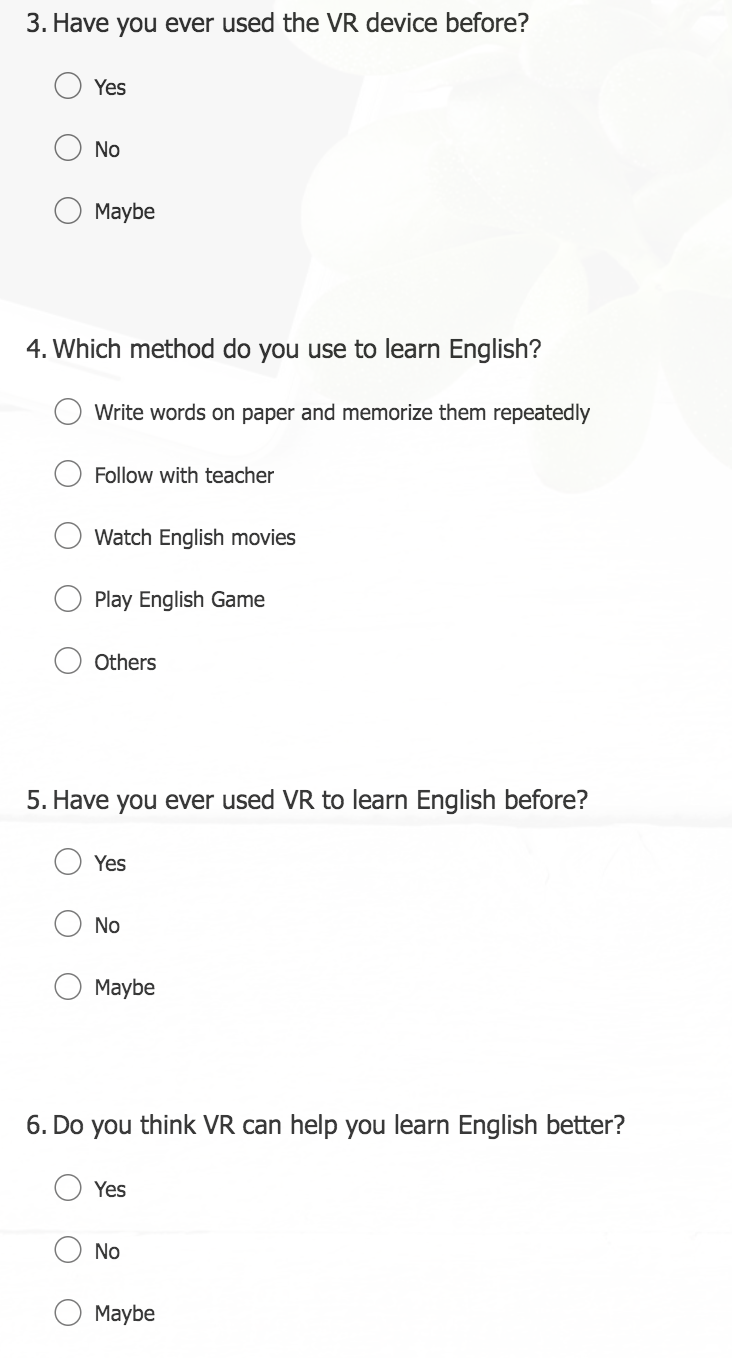
\includegraphics[width=10cm, height=16cm]{pictures/InfoSurvey.png}
 \caption{Before the start of experiment, collect basic user information. Details can be found in \url{https://forms.office.com/pages/responsepage.aspx?id=Aoi1r3r_sUurITZ_8uz8i-wNJqGnXWFBm8ENsVgdP6FUMFFIOEpJUk5VOE9CVkgzSzlLRFlXMElMSi4u} }
   \label{fig:infosurvey}
\end{figure}

\begin{figure}[H]
 \centering 
 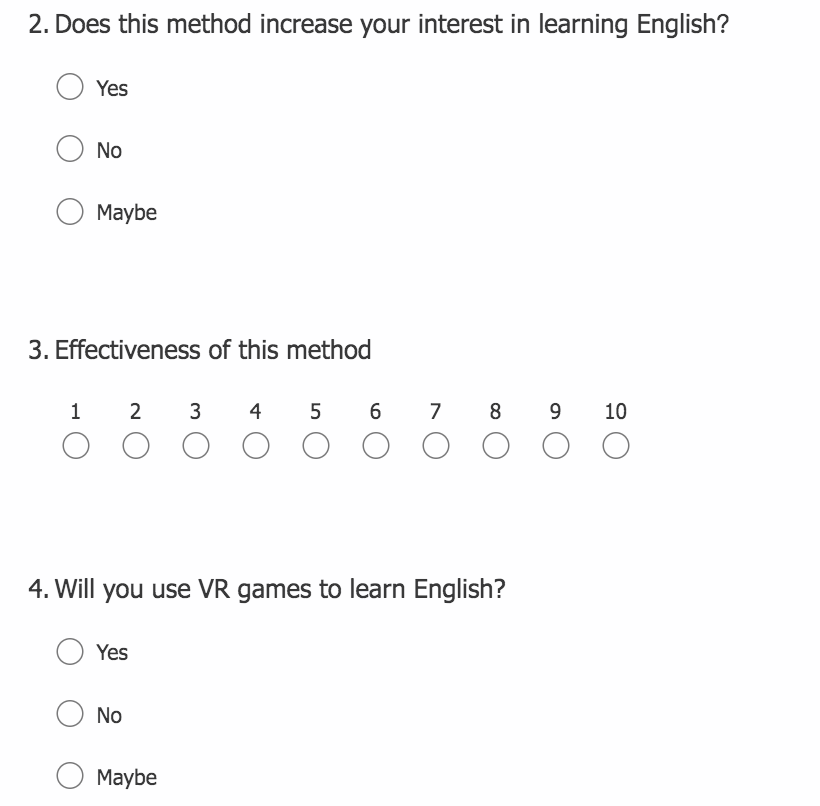
\includegraphics[width=\columnwidth]{pictures/PostPref.png}
 \caption{After the experiment, get feedback from users. Details can be found in \url{https://forms.office.com/pages/responsepage.aspx?id=Aoi1r3r_sUurITZ_8uz8i-wNJqGnXWFBm8ENsVgdP6FUMk1aNkw3QlRHMFNCRDFOUzJER0xXVzhSVy4u} }
   \label{fig:postpref}
\end{figure}
\section{Game Design}
Overall, the VR Crossword Game is divided into five scenes, they are Start, Enter ID, Version select, Learning, and Gaming \cite{lin2007implementation}. The participants will start with Start scene, and the researcher will give them ID, once they enter their ID, they need to choose a topic, each topic has different kinds of words, after this, they need to learn the words in this topic, and they start to play the VR game once they are ready.
\subsection{Preparation}
Some preparatory work is required before participants enter the game. The subjects will see three interfaces, namely the theme interface, the Enter ID interface and the version selection interface.
\begin{figure}[H]
 \centering % avoid the use of \begin{center}...\end{center} and use \centering instead (more compact)
 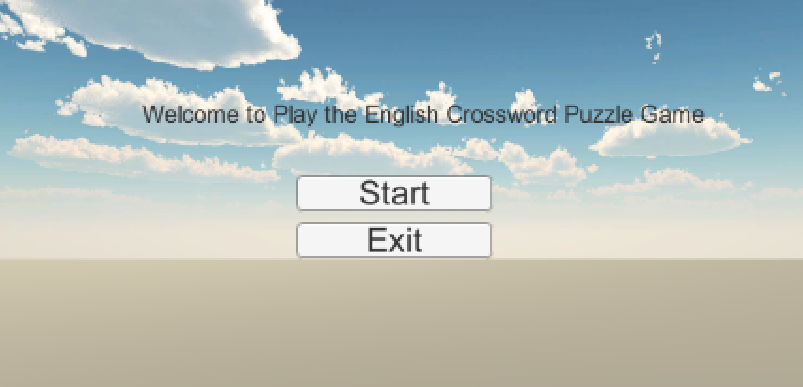
\includegraphics[width=\columnwidth]{pictures/startScene.png}
 \caption{Start Scene, choose start or quit.}
  \label{fig:start}
\end{figure}

\subsubsection{Start}
After the participants open the VR game, the first interface they will see is the Start interface (see\autoref{fig:start}). The main purpose of setting the game start interface is to make the participants adapt to the VR world and VR controller. Participants need to use the trigger button in the VR controller to click the start button. Participants can also use this interface to understand how to use others buttons on the VR controller. If the user is not ready to participate in the experiment or have any other questions, they can also  the exit button.

\subsubsection{Enter ID}
In order to record data conveniently and protect the privacy of users, researchers will provide an ID for the participants. Participants need to enter the ID into the game to record. Participants can also use this scene to learn how to use VR controllers.

\subsubsection{Version}
This game will provide three versions. Participants need to choose the version according to the requirements of the researcher. There are 5 words in each version. The five words have different degrees of difficulty. However, the overall difficulty of each version is the same. The experiment chose food as the vocabulary theme. Participants can enter the learning scene after clicking on the version.

\begin{figure}[H]
 \centering 
 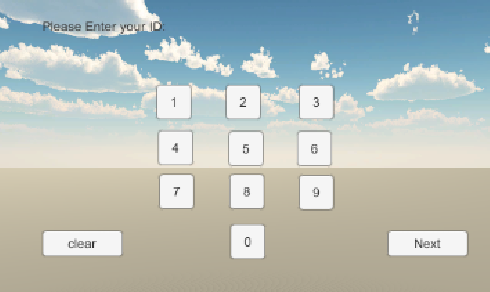
\includegraphics[width=\columnwidth]{pictures/Enter ID.png}
 \caption{Enter ID Scene. Participants will enter the ID provided by the researcher.}
 \label{fig:enterid}
\end{figure}

\begin{figure}[H]
 \centering % avoid the use of \begin{center}...\end{center} and use \centering instead (more compact)
 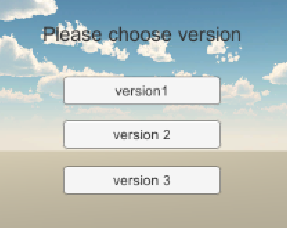
\includegraphics[width=8cm, height=6cm]{pictures/Version.png}
 \caption{Version Scene. Participants will choose the version according to the researcher's requirements..}
   \label{fig:verion}
\end{figure}
\subsection{Learning Scene}
The words in the Learning scene will appear in the game later, so participants need to remember all the words in the Learning scene.  In the current scene, an English explanation of the word appears on the panel along with the word, and participants simply drag the VR controller up and down to view all the words. 
\begin{figure}[H]
 \centering 
 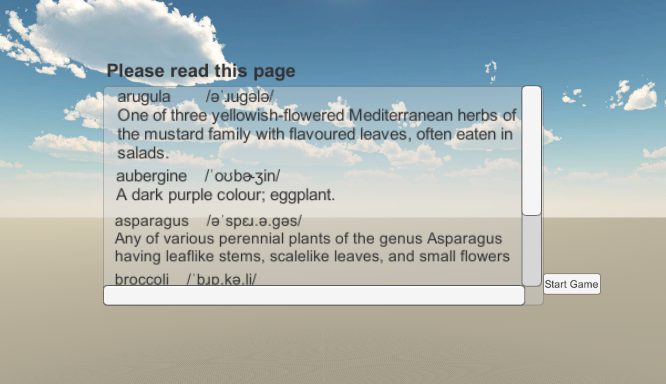
\includegraphics[width=\columnwidth]{pictures/LearningScene.png}
 \caption{Learning Scene, scroll up or down to browse multiple words.}
   \label{fig:learning}
\end{figure}
\subsection{ Game Scene}
\begin{figure}[H]
 \centering
 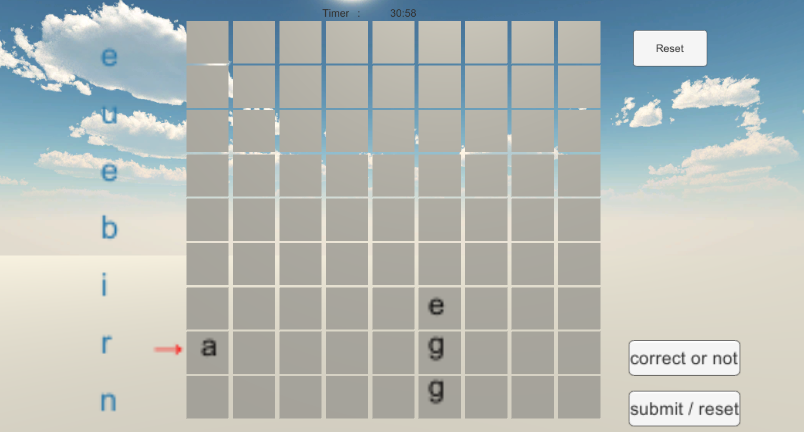
\includegraphics[width=\columnwidth]{pictures/GameScene.png}
 \caption{Game Scene, choose a letter with the controller and put it on preferred chessboard grid.}
 \label{fig:5}
\end{figure}
In the game scene, there are several reminders(Timer, arrows) to remind the participants what need to do. The board starts with the word 'egg' in the center, then generates a letter A on the second-to-last row to the far left, with a red arrow indicating which direction to enter the word. After the participants input the current word, they need to click the submit/ Reset button first, which is used to upload the current word to the background, and then click the correct or NOT button to check whether the word input is correct. If the input is wrong, they need to re-input the word, otherwise the letters just entered will be fixed on the board.  And appear the next word prompt letter and input direction. After the participants input the current word, they need to click the submit/ Reset button first, which is used to upload the current word to the background, and then click the correct or NOT button to check whether the word input is correct. If the input is wrong, they need to re-input the word, otherwise the letters just entered will be fixed on the board.  And appear the next word prompt letter and input direction.  When all the correct words are entered, ***** appears to prompt participants that the experiment has been completed, and the 'Congratulation' appears.  

\begin{figure}[H]
 \centering
 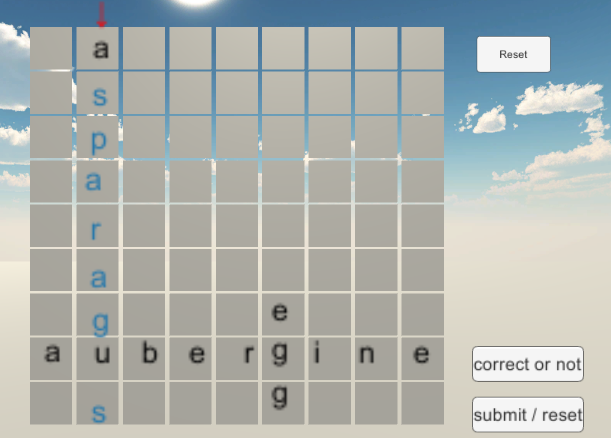
\includegraphics[width=\columnwidth]{pictures/Ingame.png}
 \caption{Game Scene, when the first word is finished}
 \label{fig:7}
\end{figure}
\subsubsection{Letter pool}
Letters are stored in the letter pool, which has the same amount of letters as the longest letter in the word set. When the longest word is present, all occurrences of Letter pool words are used; otherwise, Letter pool will generate interfering letters. Furthermore, the letters generated in the letter pool are not ordered alphabetically according to the word, thus participants must select on their own how to arrange the letters on the chessboard.(see \autoref{fig:5}).If a participant enters letters in the wrong order, the words in the letter pool go back to where they were before, which is restore.  
\subsubsection{map}
A map is made up of 9 by 9 planes(see \autoref{fig:5}), each with a space between them to distinguish the intervals.  The board is used to place letters in the letter pool, and in the flow of the game, players must first click on the letter in the letter pool and then click on the board to move the letter.  Each plane in the board has a tag on it called a map, because moving letters is done by rays in Unity.  
\subsubsection{submit/reset}
The Submit button uses 4 scripts to realize its function. When we click the Submit button, we need to call the word array(generated in "List generate script") that we input before clicking. If the input is correct, the word array will be emptied and the array index will increase by 1.  Conversely, if the input is incorrect, the word array is emptied, but the index is not increased.  The index of the array will be obtained by calling function in the "index" script, which is also attached to the Submit button. Similarly, as I mentioned in the Letter Pool section, the position of words in the Letter pool is also restored by the Submit button. However, regardless of whether the words are correctly typed, letters in the Letter pool need to be restored because the user will continue to input letters.
\subsubsection{correct or not}
When we click Correct or not, the system will invoke an animation script to determine whether the word entered is Correct or not\cite{bouvier2019advanced}. The principle is to obtain the index in the array. If the input is not Correct, the animation will not jump to next one.
\begin{figure}[H]
 \centering
 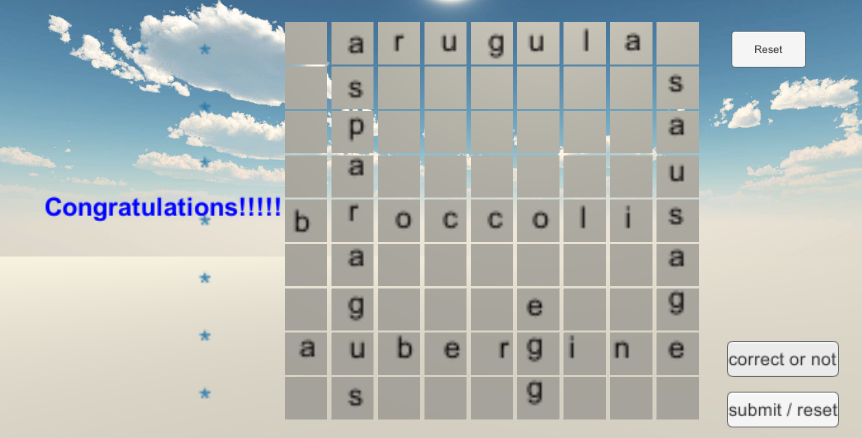
\includegraphics[width=8cm, height=5cm]{pictures/Gamefinish.png}
 \caption{Game Scene, the game finishes.}
 \label{fig:8}
\end{figure}
\begin{figure}[H]
 \centering 
 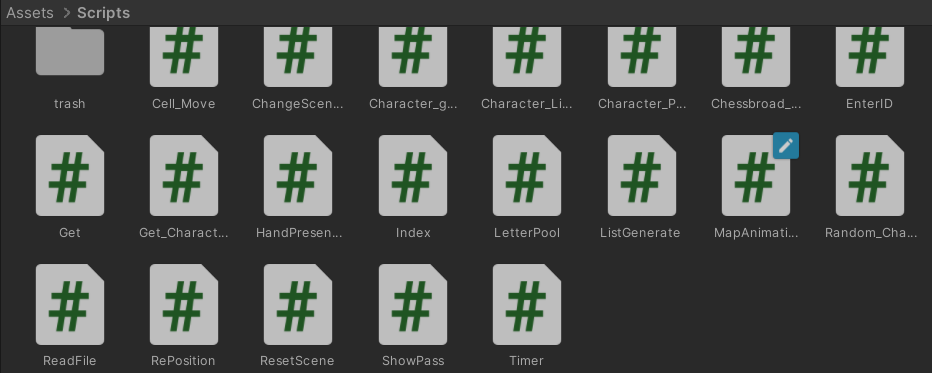
\includegraphics[width=\columnwidth]{pictures/Scripts.png}
 \caption{All of scripts we designed.}
   \label{fig:scripts}
\end{figure}
\subsubsection{Animation}
In order to help participants use the game better. Because some participants are not familiar with VR, they will place letters in inaccurate places. So we created animations to help participants better complete the game. After users complete the word spelling task, black words will appear, and these words cannot be moved.
\begin{figure}[H]
 \centering
 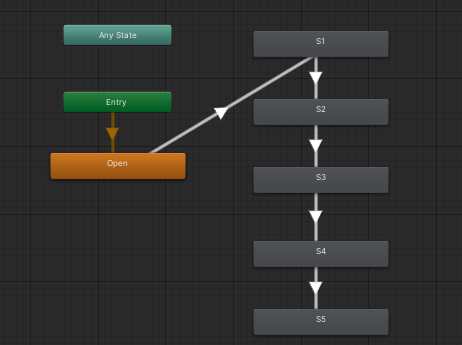
\includegraphics[width=\columnwidth]{pictures/animation.png}
 \caption{Animations. Orange 'Open' is the first animation when the player open this game. Whenever the player successfully spells a word, it will jump to the next animation, such as S1, S2, S3, S4 and S5.}
 \label{fig:9}
 
\end{figure}
\begin{figure}[H]
 \centering
 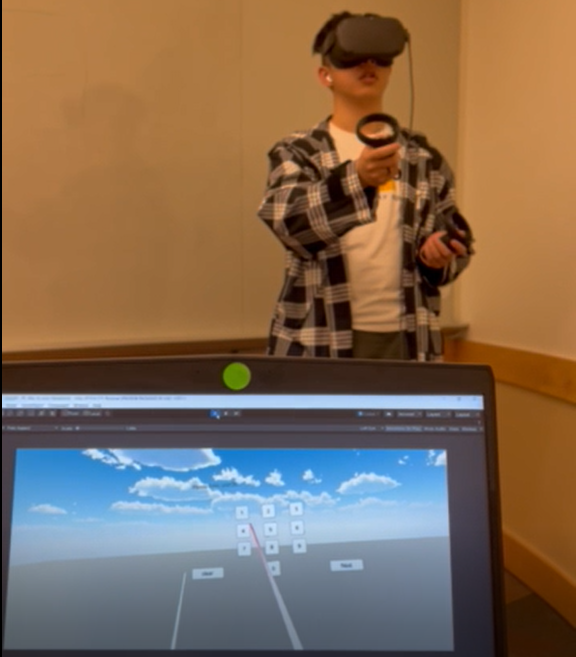
\includegraphics[width=8cm, height=9cm]{pictures/playthegame.png}
 \caption{The researcher is playing the game.}
 \label{fig:playthegame}
\end{figure}

\section{Experiments and Results}
This experiment adopted the method of control experiment. Participants need to take part in two sets of experiments. The experiment content of the control group is to complete the Crossword puzzle game in the real world \cite{derakhshan2015effects}. The experimental content of the experimental group is to complete game tasks in the VR world. Participants need to fill in the post-survey with their preferences and ideas after completing the two sets of experiments. In the experiment, the two most important variables are the independent variable and the dependent variable. In this project, the independent variables are mainly divided into the personal information of the participants, the way of the game, and the environment of the experiment(see \autoref{tab:independent}). The experiment is mainly divided into three dependent variables. The first is the accuracy of the participants during the game, and the second is the preference of the participants. The third is the time spent participating in each experiment (see \autoref{tab:dependent}).
\subsection{Participants}
The number of participants in this experiment is 9 people. Four of them are between 18-25 years old, and five are between 26-30 years old. Among them, 4 women participated in the experiment and 5 men. In addition, more than half of the participants have used VR equipment, but no one has used VR to learn English. According to the pre-survey survey results, 50 percent of participants questioned the effectiveness of using VR to learn English. One of its participants thought that using VR to learn English words is very impractical. After analyzing the results of the survey on the study habits of the participants, it is found that different people use different methods to learn English. But no one has ever used a VR device to learn English.
\begin{table}[H]
  \caption{Independent Variable}
  \label{tab:independent}
  \scriptsize%
	\centering%
  \begin{tabu}{%
	r%
	*{7}{c}%
	*{2}{r}%
	}
  \toprule
   Factor(IV) & Levels(Test conditions)\\
  \midrule
   Personal Information & Age, English Ability, Favorite Learning method \\
   Game environment & Real world, VR\\
   \bottomrule
 \end{tabu}
\end{table}

\begin{table}[H]
  \caption{Dependent Variable}
  \label{tab:dependent}
  \scriptsize%
	\centering%
  \begin{tabu}{%
	r%
	*{7}{c}%
	*{2}{r}%
	}
  \toprule
   ID & Dependent Variable \\
  \midrule
  1 & the accuracy of the participants during the game \\
  2 & the preference of the participants\\
  3 & the time spent participating in each experiment\\
  \bottomrule
  \end{tabu}%
\end{table}

\begin{figure}[H]
 \centering
 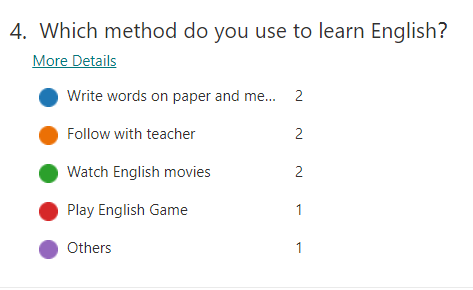
\includegraphics[width=8cm, height=5cm]{pictures/SurveyInfo.png}
 \caption{pre-suvery for getting personal information. This is the forth question which is "which method do you use to learn English?".}
 \label{fig:animation}
\end{figure}
\begin{figure}[H]
 \centering
 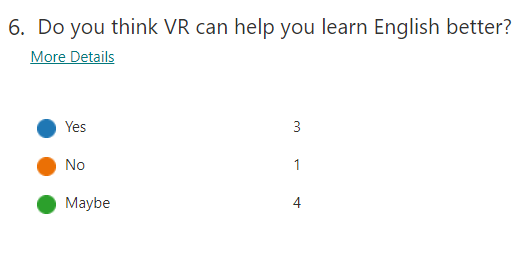
\includegraphics[width=8cm, height=5cm]{pictures/survey2.png}
 \caption{Pre-survey: Do you think VR can help you learn English better?}
 \label{fig:9}
\end{figure}
\subsection{Procedure}
\subsubsection{Real world}
Participants need to complete game tasks in the real world before they start using VR devices to learn English \cite{dewi2017effect}. Participants first need to complete the pre-survey. After that, the researchers will imitate the prompts in the real game to help participants complete the spelling of the words one by one. And in the process of completion, record the number and time of spelling mistakes by participants. Participants need to complete the Post-survey after completing the game task.
\begin{figure}[H]
 \centering
 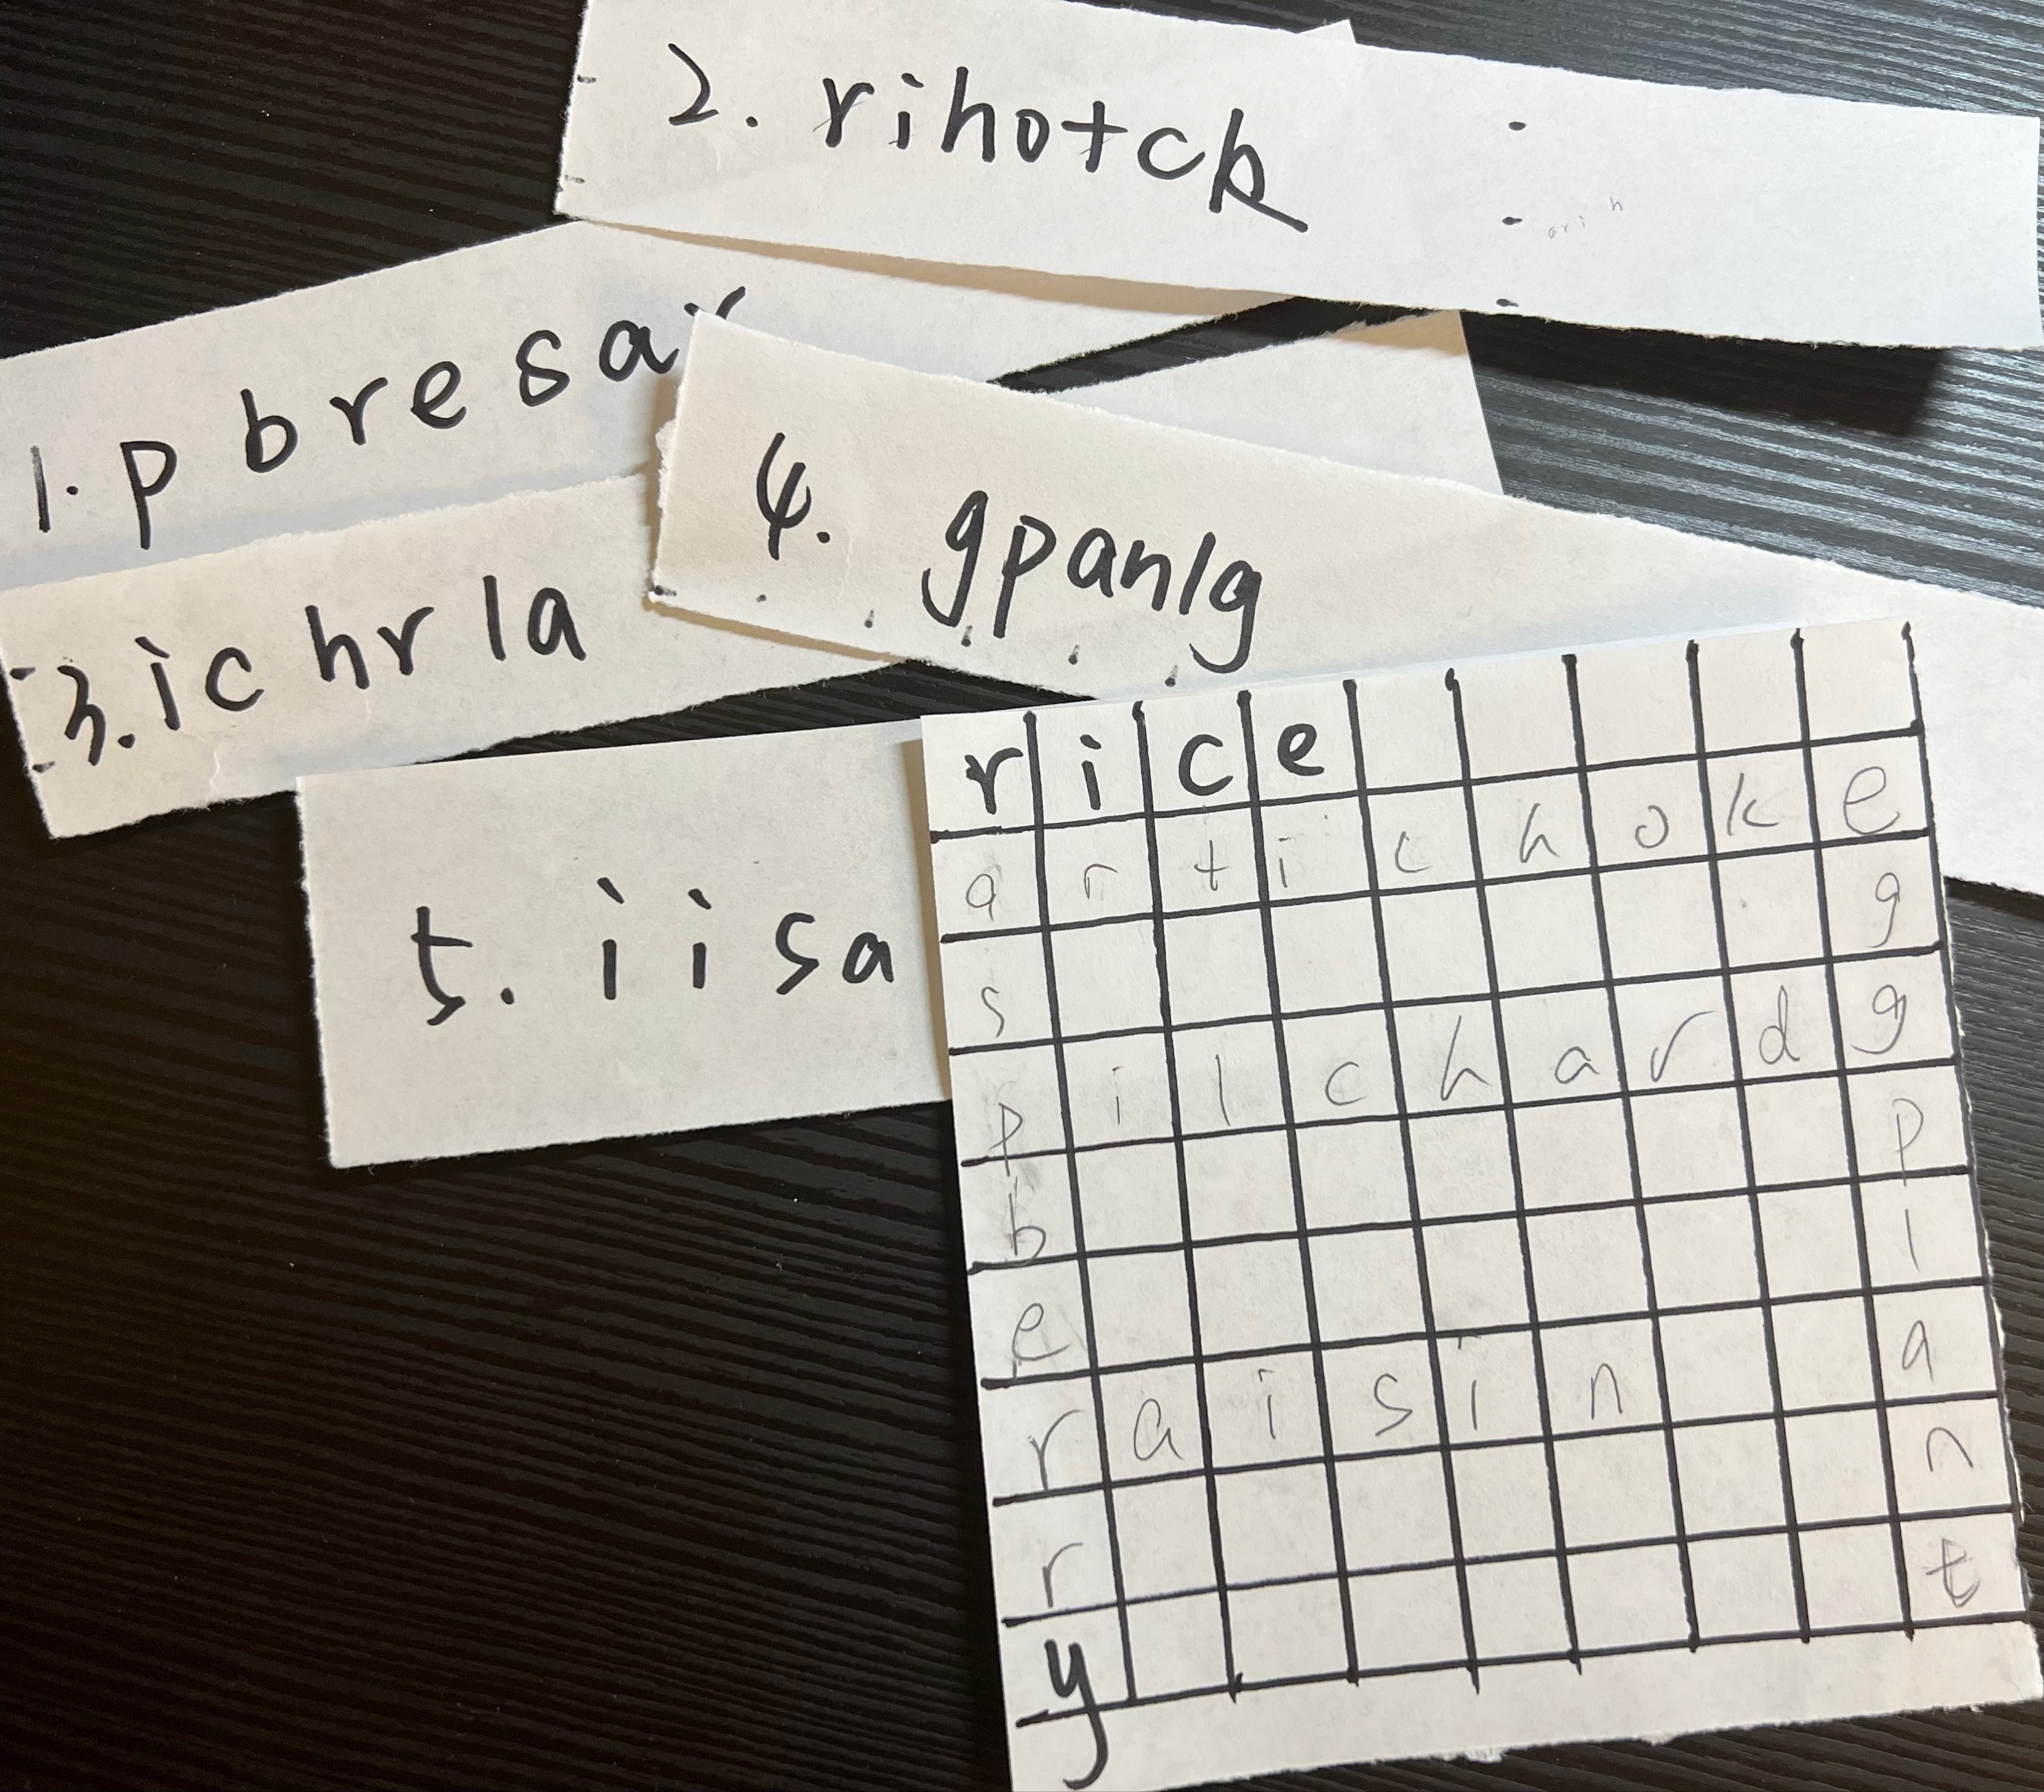
\includegraphics[width=6cm, height=6cm]{pictures/Real World.png}
 \caption{Crossword game on paper. Players will use pencils to spell words on paper. Researchers will provide letter bars one by one according to the participant’s game progress. For example, number 1 is the letter required for the first word that needs to be spelled to participate in the combination.}
 \label{fig:realworld}
\end{figure}
\subsubsection{VR world}
Participants need to complete the Pre-survey related to VR game content before starting the game. Participants will wear Oculus Quest VR headset and use the handle to complete the game. Participants need to start the game successfully according to the game prompts and the guidance of the researchers. After starting the game, the researcher will not give participants any more prompts. Participants can only spell the correct words according to the prompts in the game. Participants have only three opportunities to spell each word during the process of participating in the experiment. If all three spellings are wrong, the researcher will directly give the correct answer and list this word as a "unsuccessful" word. After completing all the experiments, participants need to complete a preference survey. This survey will help researchers better understand the participants’ thoughts on the two experiments.
\subsection{Result and Evaluation}
\subsubsection{Compare the difficulty of the two versions}
In order to prevent participants from retaining real-world word memories when conducting VR experiments, we prepared different versions for different experiments. In order to prove that the difficulty of the two versions is the same, we collected participants' initial awareness of the different versions. Among them, the average value of version 1(for VR World) is 5.625. The average value of version 2(for Real World) is 5.75. The initial familiarity of the users of these two versions is similar, so we believe that there is a certain degree of comparability between the two versions. The data of the two versions can be compared.

The table of Raw Data is the result about both experiments(see \autoref{tab:raw data}).P-ID refers to Participant-ID. P-V1 score refers to Pre-Version1 score. Po-V1 score is the abbreviation of Post-Version1 score. P-V2 score is refers to Pre-Version2 score. Po-V2 score is the abbreviation of Post-Version2 score. V1++ and V2 ++ refers to Version 1 improvement and Version 2 improvement.V1 ER refers to  Version Error Rate. 
\begin{figure}[H]
 \centering
 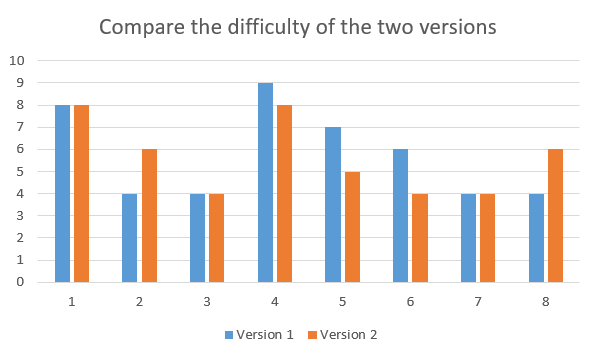
\includegraphics[width=8cm, height=6cm]{pictures/Compare.png}
 \caption{Compare Plot.}
 \label{fig:compare}
\end{figure}

\begin{table}[H]
  \caption{Raw Data}
  \setlength{\arrayrulewidth}{0.5mm}
\setlength{\tabcolsep}{2pt}
  \label{tab:raw data}
  \scriptsize%
	\centering%
  \begin{tabu}{%
	r%
	*{7}{c}%
	*{2}{r}%
	}
  \toprule
   P-ID & P-v1 score & Po-V1 score & v1 ++& V1 ER & P-V2 Score & Po-V2  & V2 ER & v2 ++\\
  \midrule
  1 & 8 & 10 & 2&0.267& 28 & 10 & 0.4&2\\
  2 & 4 & 7 & 3&0.267 &6 & 7 & 0.33 &1\\
  3 & 4 & 10 & 6& 0.4 & 4 & 10 & 0.33&6\\
  4 & 9 & 10 & 1&0.4 & 8 & 10 & 0.2&2\\
  5 & 7 & 10 & 3&0 & 5 & 10 & 0&5\\
  6 & 6 & 8 & 2&0.4 & 4 & 8 & 0.467 &4\\
  7 & 4 & 9 & 5&0.6 & 4 & 9 & 0.2&5\\
  8 & 4 & 9 & 5&0.2 & 6 & 10 & 0.133&4\\
  \bottomrule
  \end{tabu}%
\end{table}

\subsubsection{Control Group}
\begin{enumerate}
\item Compare Pre-Survey and Post-Survery of Version 1.
According to the content shown in the figure 16 (see \autoref{fig:compare version1}), it can be found that most of the participants can recite words very well, although they still use the traditional methods. In addition, the basic English skills of Participants No. 2 and No. 3 are not very strong, but they can still get a high score in the end by using traditional methods. It is obvious that traditional methods have far-reaching influence on students. Although some participants said that using traditional methods does make them feel a lot of pressure, but it is indeed a very effective method. They are also always looking for better ways to recite words.
  \item Analysis the Error Rate.
    According to the results of Version 2 error rate in Table (see \autoref{tab:raw data}), the error rate of a lot of participants is not high, which is the same as the results of pre-survey and Post-survey. Participant No. 5 has an error rate of 0. This participant has a very strong basic learning ability. The traditional learning method is very suitable for him.
\end{enumerate}

\subsubsection{Experimental Group}
\begin{enumerate}
  \item VR crossword game result analysis. 
  
   In this study, we use ANOVA test(Analysis of variance
) to evaluate the improvement of effectiveness \cite{anderson2004regression}. As in the \ref{fig:realworld} and post-survey result shows, we pasteurized the familiarity to words using the word pre-survey score. Our null hypothesis is that VR crossword game does not improve users' familiarity with words, i.e. VR crossword game can not help users memorize English vocabularies. There are two groups with 16 result values, thus the first degree of freedom is 1 and second degree of freedom is 14. Sum of square within groups is 39 while the sum of square is 49. Based on the previous data and F score algorithm\cite{st1989analysis}\cite{chakraborty2016sequential}, 
$$Fscore=\frac{\textrm{Sum of square within groups}/DOF1}{\textrm{Sum of square between groups}/DOF2}$$
Assume $p<0.05$, check F distribution table $F(1,14)=4.6$. The F score is $17.59>F(1,14)$, thus we reject the null hypothesis. The above data and analysis proved that VR technique can effectively augment the memory ability of users.

    \item Analysis the Error Rate.
    The error rate of the experimental group was 0.316. After observing the participants, they were affected by many factors. In our interview, one participant said that he would become anxious because he was not used to VR operation, thus affecting the memory efficiency of words, and sometimes even forgetting what words he had memorized. Therefore, we speculated that participants would be less efficient in moving words for a long time, and that wearing VR would have an unnatural feeling, which would also affect participants' feelings, and sometimes even affect efficiency and experiment accuracy.
    
\end{enumerate}

\subsubsection{Compare results of two groups}
\begin{enumerate}
  \item Comparison two groups with ANOVA result.
    
    Based on the score improvement made by two different groups, we analyzed the validity of VR crossword game compared to real world physical game. Apply the above ANOVA analysis method on improvement data\ref{tab:raw data} \cite{10.1145/206944.207007}\cite{DRISCOLL1996265}. Our hypothesis is that the English word memorize ability improvement made through VR crossword game is less than it made through playing physical world game.Sum of square within groups is 43.75 while the sum of square is 44. Assume $p<0.05$, the F score is $0.08<F(1,14)$, thus we accept the null hypothesis\cite{driscoll1996robustness}. Which indicates that the real world crossword game outperformed the VR application we developed in boosting users' memorization of English\cite{fata2016down}.
    
  \item By comparing VR test and paper test, the error rate of VR test is 0.316, while that of paper test is 0.2575. It can be obviously found that paper test has a lower error rate. Here's what we can guess about this result: People doing VR experiments will make mistakes because they are unfamiliar with the operation. The operation of VR is complicated, which reduces the efficiency of learning words. When people play VR for the first time, they will feel excited or nervous. We guess that both positive and negative emotions will affect the efficiency of learning words. In the paper test, the participants were allowed to spell words out of order, but in the VR test, the words had to be spelled backwards. We speculated that this rule might also affect word memory or spelling efficiency. We found that people are more used to this more traditional method of memorizing words. According to the post-survey, more people want to use the more traditional method of memorizing words, although they think VR is a novel method of memorizing words.
  \item The average Controlled Group completion time was around five minutes, while the average VR completion time was around 13 minutes. Part of this is due to the lack of VR proficiency and familiarity with VR gamepads. Through the records, we found that participants spent a significant amount of time moving letters, resulting in a significant difference in the time spent moving text
    
    \begin{figure}[H]
 \centering
 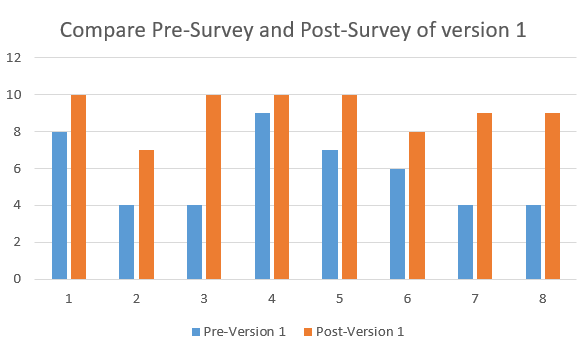
\includegraphics[width=8cm, height=6cm]{pictures/Compare Version 1.png}
 \caption{Compare Pre-Survey and Post-Survey of Version 1 Plot. Version 1 is the experiment for VR world.}
 \label{fig:compare version1}
\end{figure}

\begin{figure}[H]
 \centering
 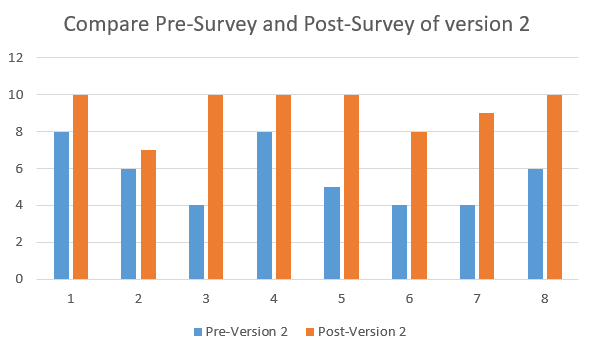
\includegraphics[width=8cm, height=6cm]{pictures/Compare Version 2.png}
 \caption{Compare Pre-Survey and Post-Survey of Version 2 Plot. Version 21 is the experiment for Real world.}
 \label{fig:computer version2}
\end{figure}
\end{enumerate}


\section{Limitation}
In this experiment, there are several limitations which caused by program design limitation. 
\begin{enumerate}
    \item Some letters in the letter pool, like "i" or "l" are too slim to click,We should increase the size of the decision area to make it easier for participants to click. this limitation leads to a loss of user experience and slow down the game.
    \item The survey was not rigorous. One participants said that "The boundary of familiar and unfamiliar is not clear." She advises us to add an option "familiar but can not spell" in the survey. This would helps the survey to be more accurate.
    \item The test words of VR and real world are different, if the words are the same, the results would be more accurate. But we do not have enough participants, so we can not do enough controlled experiments.
    \item No tutorial, participants spent plenty time on getting familiar with VR device. So this likes the first limitation, it also slow down the game, makes the experiment not accurate.
    \item There is no clear goals of this game in the game scene, so this makes some participants do not know what to do. And this also slow down the game.
    \item Some participants would double click the letters no matter on the letter pool or on the chessboard. Because sometimes participants are not sure about whether they have clicked the letter or not. And when they click the chessboard, because the size of the decision area of other letter which has been settled on the chessboard is too large, the participants would click that letter by accident. 
    \item For those participants who use VR device first time, some of them are nervous. This would influence their performance. Because when we do the dictation on the paper, we will not have such feeling like nervous or excited, I think these kinds of feeling would have negative effect on us.
\end{enumerate}
\section{Discussion}
\subsection{Real World Crossword Game}
In the control group, eight people who took the paper test learned a total of 29 words, so each person learned almost 3.6 words. In the experimental group, eight people learned a total of 27 words after undergoing VR word learning, so each person learned 3.4 words. Overall, the results of the control group were better than those of the experimental group. People said that it was easier to perform word solitons on paper, "it is much easier to move letters on paper than in VR, and I can think coherently when testing on paper, and I can concentrate better." Others said: "When I use VR to recite words, I will be attracted by objects other than words, such as the virtual sun is beautiful. I will sometimes be distracted by these scenes, which reduces my efficiency in learning words." Through the survey of these subjects, we found that VR scenes would bring different feelings to people, but these feelings would distract participants, thus reducing efficiency. In the post-survey, most people said they would still use the traditional method of reciting words rather than using VR. According to the final experimental data, participants' intuitions were correct, and the efficiency gains from VR were not as high as those from the words solitons on paper.
\subsection{VR Crossword Game}
In the experimental group, eight people learned a total of 27 words after undergoing VR word learning, so each person learned 3.4 words. In the control group, eight people who took the paper test learned a total of 29 words, so each person learned almost 3.6 words. Overall, the results of the control group were better than those of the experimental group. In terms of time, VR group average available in 13 minutes, by observing the participants of the experiment process, we found that the participants spent a lot of time on the mobile letter, we also interviewed some of the participants, they said "mobile letter is a time-consuming work, sometimes because mobile current letter to forget what is the next to the mobile letter." At the same time, we also asked them which method of memorizing words they preferred, and almost all participants chose to use traditional paper-based words. "VR sometimes makes it hard for me to concentrate on memorizing words, and the virtual environment of VR distracts me," said one of the testers. Therefore, we speculate that the virtual environment will also make people feel unreal, which will reduce people's concentration and thus reduce efficiency.

\section{Conclusion}
In this experiment, we found that Crossword game is very effective in learning English words, which can greatly increase the fun of the game and reduce people's anxiety and boredom when reciting words. Experimental data show that although VR can improve the efficiency of memorizing words, the efficiency improvement it brings is not as high as the control group, that is, the paper test. People more bias from the traditional method of memorizing words, we speculate that the test on the paper, will reduce the invalid behavior of participants, comparing the VR group, test group will not be used on the paper the uncomfortable feeling when VR or excitement, so a paper test group efficiency will be higher than the VR group, considering the VR group need again with handle in VR games move the letters, Thus, participants' emotions may fluctuate due to inefficient letter movement rates. In addition, through the experimental data, we found that the paper tests the small errors, we guess is we will not rule the experimenter spelling words on the paper order, but in VR, participants in the input sequence is must, in turn, input the correct sequence of letters, so this is not convenience may results in the decrease of the efficiency of the participants spelling words. Through the questionnaire survey, we found that people are not averse to using VR as a new way to memorize words, but almost no one will actively choose to use VR to memorize words, and people still prefer to use more traditional methods to memorize words. This is similar to the experimental results. Our conclusion is that VR is an effective new way to memorize words, but the efficiency improvement is not as high as the control group.

\section{Future Work}
Different game modes can be added to make the game more interesting and playable. For example, a timing mode can be added, so that testers who complete the test within a specified time can get corresponding points to advance to the next level, and they can get rewards corresponding to the number of completed tests.
Adding different language patterns, since the purpose of this is to remember English words, so in the future of VR games, developers can try other languages in China \cite{jiang2020english}. For example, words solitaire is very popular, so maybe this project can be better help Chinese learning, namely to learning other languages have greater help\cite{chun2003computer}.
More abundant word themes are added. Since this project only has food words, more word themes can be added in the future to enhance the fun of the game and make participants feel stronger gameplay.



%% if specified like this the section will be committed in review mode
% \acknowledgments{
% The authors wish to thank A, B, C. This work was supported in part by
% a grant from XYZ.}

%\bibliographystyle{abbrv}
\bibliographystyle{abbrv-doi}
%\bibliographystyle{abbrv-doi-narrow}
%\bibliographystyle{abbrv-doi-hyperref}
%\bibliographystyle{abbrv-doi-hyperref-narrow}

\bibliography{template}
\end{document}
